\documentclass[12pt]{article}
\usepackage[utf8]{inputenc}
%\usepackage{csquotes}
\usepackage{graphicx}
\graphicspath{ {pictures/} }
\usepackage{caption}
\usepackage{subcaption}
\usepackage[a4paper,width=150mm,top=25mm,bottom=25mm,bindingoffset=6mm]{geometry}
\usepackage[english]{babel}
\usepackage{amsthm,etoolbox, amsmath, amssymb}
\usepackage{enumitem}   
\usepackage[nottoc]{tocbibind}
\usepackage{hyperref}
\usepackage{wrapfig}
\usepackage{color} 
\usepackage [autostyle, german = quotes]{csquotes}
\usepackage{tikz}
\usepackage{pgffor}
\usepackage{listings}
\usepackage{fancyhdr}
\MakeOuterQuote{"}

\AddToHook{cmd/section/before}{\clearpage}

\theoremstyle{plain}
\newtheorem{thm}{Theorem}
\newtheorem{lem}[thm]{Lemma}
\newtheorem{prop}[thm]{Proposition}
\newtheorem{cor}[thm]{Corollary}

\theoremstyle{definition}
\newtheorem{definition}[thm]{Definition}
\newtheorem{ex}[thm]{Example}
% \AtBeginEnvironment{ex}{
%   \pushQED{\qed}\renewcommand{\qedsymbol}{\par\noindent\rule{0.33\textwidth}{0.2pt}}
% }
% \AtEndEnvironment{ex}{\popQED\endexample}
\theoremstyle{remark}
\newtheorem{rem}[thm]{Remark}

\makeatletter
\@addtoreset{thm}{section}% Reset theorem counter with every section
\@addtoreset{thm}{subsection}
\@addtoreset{thm}{subsubsection}
\newcommand{\theoremprefix}{}
\let\thetheoremsaved\thethm
\renewcommand{\thethm}{\theoremprefix\thetheoremsaved}
\let\sectionsaved\section
\patchcmd{\@startsection}{\par}{\renewcommand{\theoremprefix}{\csname the#1\endcsname.}}{}{}
\makeatother

\setlength{\jot}{10pt}
\setlength{\headheight}{15pt}

\newcommand*\circled[1]{\tikz[baseline=(char.base)]{%
            \node[shape=circle,fill=blue!20,draw,inner sep=2pt] (char) {#1};}}

\usepackage[style=alphabetic, firstinits=true, backend=biber, sorting=nyt, doi=false, isbn=false, url=true, maxbibnames=99]{biblatex}
\DeclareNameAlias{default}{family-given}
\addbibresource{references.bib}

\title{Thesis Title}
\author{Author Name}
\date{Day Month Year}

\setlength\parindent{0pt}

\begin{document}
	\begin{titlepage}
	\begin{center}
		\vspace*{1cm}
		
\includegraphics{TU_Logo_kurz_1c_schwarz.eps}\\
		\Large
		Technische Universität Berlin\\
		Institut für Mathematik
		\vspace*{1cm}



		\Huge
		\textbf{Numerischer Wertebereich}
		
		\vspace{0.5cm}
		\LARGE
		und Anwendung auf das Lax-Wendroff-Verfahren
		
		\vspace{1.5cm}
		
		\textbf{Sijun John Tu}
		
		\vfill
		
		Bachelorarbeit \\
		zur Erlangung des Grades\\
		Bachelor of Science \\
		im Fach Mathematik
		
		\vspace{0.8cm}

		
		
		Betreuerin: Frau Dr. Agnes Radl\\
		Zweitgutachterin: Prof. Dr. Tanja Eisner \\
		
	\end{center}
\end{titlepage}
	
\subsubsection*{Abstract}

    In this paper, we investigate the so-called numerical value range of a linear, bounded operator in a Hilbert space. Similar to the spectrum of an operator, the numerical range of values helps to determine certain properties of the corresponding operator to be investigated. In doing so, we will often encounter relations between there two invariants. The main objective of this section is the so-called Power Inequality, a statement about the numerical radius of powers of an operator, as well as the norm property of the numerical radius. In particular, an algorithm is presented and implemented, which numerically approximates the numerical value for a finite-dimensional operator. In the final chapter of the thesis, an application of the numerical value range in numerical mathematics is considered.


	\thispagestyle{empty}
\section*{Eidesstattliche Erklärung}

Hiermit erkläre ich, dass ich die vorliegende Arbeit selbstständig und eigenhändig sowie ohne unerlaubte fremde Hilfe und ausschließlich unter Verwendung der aufgeführten Quellen und Hilfsmittel angefertigt habe.\\

Die selbstständige und eigenhändige Anfertigung versichert an Eides statt:\\\\\\\\\\
Berlin, den \today \\[5cm]
\rule{10cm}{0.4pt}\\
Sijun John Tu
	\tableofcontents
	\thispagestyle{empty}
	% \addtocontents{toc}{\protect\thispagestyle{empty}}
	\setcounter{page}{0}

	
\section*{Notation}
Mathematical conventions and notation used in this thesis:

\begin{center}
    \renewcommand{\arraystretch}{1.5}
    \begin{tabular}{ c l }
        
        $\mathbb{R}$ & the real numbers \\
        $\sqcup$ & disjoint set union \\
        $\mathcal{N}(\mu, \sigma^2)$ & Gaussian distribution with mean $\mu$ and variance $\sigma^2$
    \end{tabular}
\end{center}

Additionally, we introduce the following conventions to describe various elements from different mathematical objects to make the notations and their meaning as consistent as possible:

\begin{center}
    \renewcommand{\arraystretch}{1.5}
    \begin{tabular}{c l}
        $\mathcal{S}$ & set of heartbeat samples \\
        $s_i \in \mathbb{R}^L$ & seqeunce of ECG measurements \\
        $\mathcal{K}^X$ & arrhythmia detection model trained on some training data $X$


    \end{tabular}
\end{center}

	\addcontentsline{toc}{section}{Notation}

	\listoffigures

	\pagestyle{fancy}
	\fancyhf{}
	\fancyhead[L]{\leftmark}
	\fancyfoot[R]{\thepage}


	Der numerische Wertebereich und Radius werden in einem Hilbertraum-Setting für lineare und beschränkte Operatoren definiert. Daher werden in diesem Abschnitt die grundlegenden Ergebnisse und Definitionen aus der Theorie der Hilberträumen in kompakter Weise erläutert, aber ohne Beweis aufgeführt. Details können den Standardwerken zur Funktionalanalysis entnommen werden, siehe \parencite[][Kapitel 5, 6]{werner2006funktionalanalysis} oder auch \parencite[][Kapitel 1,2, 6, 7]{conway2019course}.

\subsection{Hilberträume}

Sei $\mathbb{K}$ ein Körper. Im Kontext dieser Arbeit wird $\mathbb{K}$ meistens der Körper der komplexen Zahlen $\mathbb{C}$ sein, seltener auch der Körper der reellen Zahlen $\mathbb{R}$. Üblicherwei\-se wird die Notation $\mathbb{K} \in \{\mathbb{C}, \mathbb{R}\}$ eingeführt. Auf einem Vektorraum $X$ über $\mathbb{K}$ definieren wir das Skalarprodukt als eine Abbildung, die zwei Elemente aus dem Vektorraum auf ein Element des zugrundeliegenden Körpers wie folgt abbildet:

\begin{definition}[Skalarprodukt]
    Sei X ein Vektorraum über $\mathbb{K}$. Dann ist ein Skalarprodukt auf X eine Abbildung
    \begin{align*}
        \left<\cdot ,\cdot \right> : X \times X \longrightarrow \mathbb{K} \; ,
    \end{align*}
    welche folgende Eigenschaften für alle $ x,y,z \in X$ und $a, b \in \mathbb{K}$ erfüllt: \begin{enumerate}[label=(\roman*)]
        \item Linearität im ersten Argument: \begin{align*}
            \left< a x + b y, z \right> = a \left< x , z \right> +b \left< y, z \right>
        \end{align*}
        \item konjugierte Symmetrie: \begin{align*}
            \left< x,y \right> = \overline{\left< y,x \right>}
        \end{align*}
        \item  positive Definitheit: \begin{align*}
            \left< x,x \right> \ge 0 \\
            \left< x,x \right> = 0 \iff x = 0
        \end{align*}
    \end{enumerate}
\end{definition}

Einen Vektorraum ausgestattet mit einem Skalarprodukt nennt man auch einen Prä\-hilbert\-raum. Ein Hilbertraum ist dann ein voll\-ständiger Prä\-hilbert\-raum, wobei als Norm die vom Skalarprodukt induzierte Norm betrachtet wird (man mache sich bewusst, dass es sich dabei wirklich um eine Norm handelt!).

\begin{definition}[Hilbertraum]
    Sei $X$ ein Prähilbertraum mit Skalarprodukt $\left<\cdot, \cdot \right>$ und induzierter Norm $\| \cdot \| = \sqrt{\left<\cdot, \cdot \right>}$. Dann ist $X$ ein Hilbertraum, falls $X$ vollständig bezüglich $\| \cdot \|$ ist.
\end{definition}

\begin{ex} \label{ex:standard_skp}
    Das Standardskalarprodukt auf $\mathcal{H}=\mathbb{C}^n$ ist wie folgt definiert: Für Vektoren \begin{align*}
        x = \begin{pmatrix}
            x_1 \\ \vdots \\ x_n
        \end{pmatrix} \; , \;
        y = \begin{pmatrix}
            y_1 \\ \vdots \\ y_n
        \end{pmatrix}
    \end{align*}
    aus $\mathcal{H}$
    ist \begin{align*}
        \left<x,y \right> = \sum_{k=1}^n {x_k \overline{y_k}} \;\; .
    \end{align*} 
    $\mathbb{C}^n$ mit dem so definierten Skalarprodukt ist ein Hilbertraum.
\end{ex}

Nun können lineare, beschränkte Operatoren auf einem Hilbertraum definiert werden.

\begin{definition}[linearer, beschränkter Operator]
    Sei $T: \mathcal{H} \longrightarrow \mathcal{H}$ eine Abbildung auf einem Hilbertraum $\mathcal{H}$. Dann ist $T$ \begin{enumerate}[label=(\roman*)]
        \item linear, falls für alle $x,y \in \mathcal{H}$ und $a ,b \in \mathbb{K}$ gilt: \begin{align*}
            T(a x + b y) = a Tx + b Ty
        \end{align*}
        \item beschränkt, falls ein $M > 0 $ existiert, sodass für alle $x \in \mathcal{H}$ gilt: \begin{align*}
            \| Tx \| \le Mx
        \end{align*}
    \end{enumerate}
    Der Raum aller linearen, beschränkten Operatoren auf $\mathcal{H}$ wird mit $\mathcal{L}(\mathcal{H})$ bezeichnet. Ausgestattet mit der Operatornorm $\|T\| = \sup_{\|x\|=1} \|Tx\| $ ist $\mathcal{L}(\mathcal{H})$ sogar ein Banachraum, solange $\mathcal{H}$ ein Hilbertraum ist. 
\end{definition}

Falls $\mathcal{H}$ endlichdimensional ist, kann jeder lineare, beschränkte Operator mit einer Matrix identifiziert werden. Das Konzept der adjungierten Matrix kann auch für unendlichdimensionale Hilberträume verallgemeinert werden und führt auf den Begriff des adjungierten Operators.

\begin{definition}[adjungierter Operator]
    Für $T\in \mathcal{L}(\mathcal{H})$ heißt der eindeutige Operator $T^*\in \mathcal{L}(\mathcal{H})$ mit $\left< Tx,y \right> = \left< x,T^*y \right>$ für alle $x, y \in \mathcal{H}$ der zu $T$ adjungierte Operator.  
\end{definition}

Es ist nützlich, bestimmte Klassen von Operatoren in Hilberträumen näher zu betrachten, daher werden nun unitäre, normale und selbst-adjungierte Operatoren definiert.

\begin{definition}[selbst-adjungierte, normale, unitäre Operatoren]
    Ein linear, beschränkter Operator $T \in \mathcal{L}(\mathcal{H})$ heißt
    \begin{itemize}
        \item selbst-adjungiert, falls $T=T^*$
        \item normal, falls $T$ und $T^*$ kommutieren, das heißt $TT^*=T^*T$
        \item unitär, falls $T$ invertierbar und $T^{-1}=T^*$
    \end{itemize}
\end{definition}

Manchmal ist es auch hilfreich, Projektionen von einem Hilbertraum auf einen Unterraum $V$ zu betrachten. Insbesondere werden wir die sogenannte orthogonale Projektion benötigen, um ein Theorem über die Konvexitätseigenschaft des numerischen Wertebereichs zu beweisen. Die orthogonale Projektion bildet ein beliebiges Element $x$ aus dem Hilbertraum auf das eindeutige Element im Unterraum $V$ ab, sodass der Abstand zwischen diesen beiden Elementen genau dem Abstand zwischen $x$ und $V$ entspricht. 

\begin{thm}[Orthogonale Projektion] \label{thm_orth_proj}
    Sei $\mathcal{H}$ ein Hilbertraum und $V \subseteq \mathcal{H}$ ein abgeschlossener, nicht-leerer, linearer Unterraum. Dann existiert zu jedem $x \in \mathcal{H}$ ein eindeutiges Element $Px \in V$, sodass $\|x-Px\|=d(x, V)= \inf_{v\in V} \|x-v\|$. Die Abbildung \begin{align*}
        P: \mathcal{H} \longrightarrow \mathcal{H} \; \; , \; x \mapsto Px
    \end{align*}
    heißt die orthogonale Projektion von $\mathcal{H}$ auf $V$. Außerdem ist $P \in \mathcal{L}(\mathcal{H})$ und selbst-adjungiert. 
\end{thm}

\subsection{Spektraltheorie}

Das Konzept von Eigenwerten und -vektoren aus der linearen Algebra kann auch auf unendlichdimensionale Vektorräume verallgemeinert werden. Dafür werden folgende Mengen definiert:

\begin{definition}
    Sei $\mathcal{H}$ ein komplexer Hilbertraum und $T\in \mathcal{L}(\mathcal{H})$. Dann definiert man: \begin{itemize}
        \item die Resolventenmenge von $T$ \begin{align*}
            \rho(T) := \left\{ \lambda \in \mathbb{C}: \lambda -T \text{ ist bijektiv} \right\}
        \end{align*}
        \item das Spektrum von $T$
        \begin{align*}
            \sigma(T)=\mathbb{C} \setminus \rho(T)
        \end{align*}
        
        \item das Punktspektrum von $T$ 
        \begin{align*}
            \sigma_{p}(T) := \left\{ \lambda \in \mathbb{C}: \lambda -T \text{ ist nicht injektiv} \right\}
        \end{align*}
        \item das approximative Punktspektrum von $T$ 
        \begin{align*}
            \sigma_{app}(T)=\{ \lambda \in \mathbb{C}: \exists \{x_n\}_n \in \mathcal{H} \text{ sd. } \|x_n\|=1  \text{ für alle $n\in\mathbb{N}$ und } \\ 
            \|(T-\lambda)x_n \| \rightarrow 0 \text{ für } n \rightarrow \infty \}
        \end{align*}
        \item den Spektralradius von $T$ \begin{align*}
            r(T)=\sup_{\lambda \in \sigma(T)} |\lambda|
        \end{align*}
    \end{itemize}
\end{definition}

Dabei gilt folgende wichtige Inklusion \parencite[][Problem 78]{halmos2012hilbert}.

\begin{lem} \label{lem:point_approx_spec}
    Der Rand vom Spektrum ist enthalten im approximativen Punktspektrum, das heißt $\partial \sigma(T) \subseteq \sigma_{app}(T)$
\end{lem}


\subsection{Schurzerlegung}

Es ist bekannt, dass das Spektrum eines Operators invariant unter Ähnlich\-keits\-trans\-for\-ma\-tionen ist. Eine schwächere Aussage gilt auch für den numerischen Wertebereich - nämlich nur noch für unitäre Ähnlichkeitstransformationen. Diese Eigenschaft werden wir später in Proposition \ref{prop:properties_numran} zeigen. Daher ist es im Endlichdimensionalen sinnvoll, die sogenannte Schur-Zerlegung von Matrizen zu betrachten; diese erlaubt es, jede Matrix als eine unitär ähnliche obere Dreiecksmatrix darzustellen. Sie wurde 1909 von Issai Schur entdeckt und bewiesen in \parencite{schur1909charakteristischen}.

\begin{thm}[Schur-Zerlegung]
    Sei $A \in Mat_{n,n}(\mathbb{C})$. Dann existiert eine unitäre Matrix $U\in Mat_{n,n}(\mathbb{C})$ sodass 
    \begin{align*}
        U^*AU = R
    \end{align*}
    wobei $R$ eine obere Dreiecksmatrix ist.
\end{thm}

Findet man also so eine Zerlegung einer Matrix, dann lassen sich die Eigenwerte direkt von der Diagonalen von $R$ ablesen.


	
	\section{Project introduction}

\begin{frame}
    \frametitle{Machine Learning Pipeline}
    \tikz{
            \node[circle,fill=Button1,inner sep=3pt] (c) at (0,0){};
            \node[circle,fill=Button2,inner sep=3pt] (c) at (0.5,0){};
            \node[circle,fill=Button3,inner sep=3pt] (c) at (1,0){};
        }~~~~~~\textcolor{gold}{Figure: }High-level machine learning pipeline
    \begin{figure}[h]
        
        \centering
        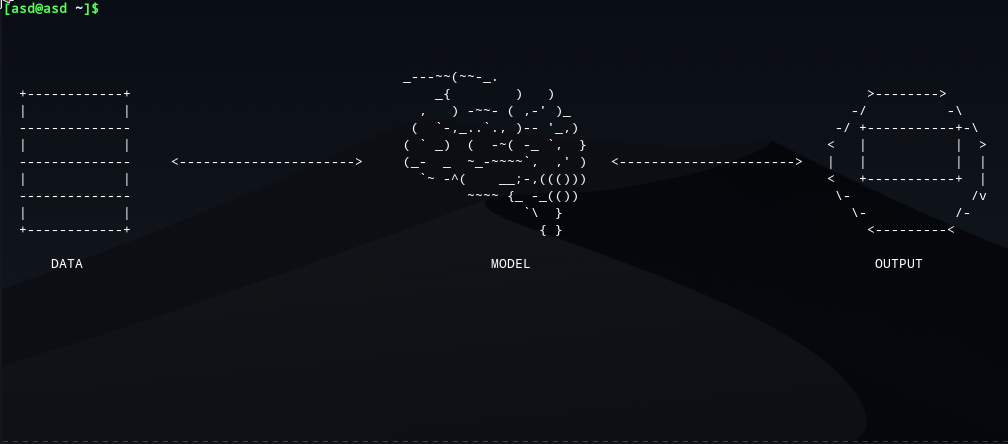
\includegraphics[scale=0.45]{ml_pipeline.png}
    \end{figure}
\end{frame}



\begin{frame}{Anomaly detection using privacy-preserving, synthetic time series data}
    
    \begin{itemize}
        \item Problem
        \begin{itemize}
            \item ML models are very \alert{data hungry}.
            \item In many cases sharing data comes with \alert{privacy risks}.
        \end{itemize}
        \item Solution:
        \begin{itemize}
            \item Promising solution: \alert{synthetic data} with privacy guarantees!
            \item Synthetic data with \alert{differential private} (DP) guarantees is a promising solution to ensure privacy independent of downstream task.
        \end{itemize}
        \item BUT:
        \begin{itemize}
            \item \alert{Privacy-Utility-Tradeoff}: Commonly, a gain in privacy results in a loss of utility. 
            \item For \alert{anomaly detection} this might not be the case (?).
        \end{itemize}
    \end{itemize}
    Goal: generate useful and privacy-preserving ECG data for anomaly detection (heartbeat arrhythmia).
\end{frame}


\begin{frame}{Structure}
    
    \begin{figure}[h]
        \begin{flushleft}
            \tikz{
            \node[circle,inner sep=3pt] (c) at (-0.5,0){};
            \node[circle,fill=Button1,inner sep=3pt] (c) at (1.0,0){};
            \node[circle,fill=Button2,inner sep=3pt] (c) at (1.5,0){};
            \node[circle,fill=Button3,inner sep=3pt] (c) at (2.0,0){};
        }~~~~~~\textcolor{gold}{Figure: }Structure of Experiment pipeline
        \end{flushleft}
        \centering
        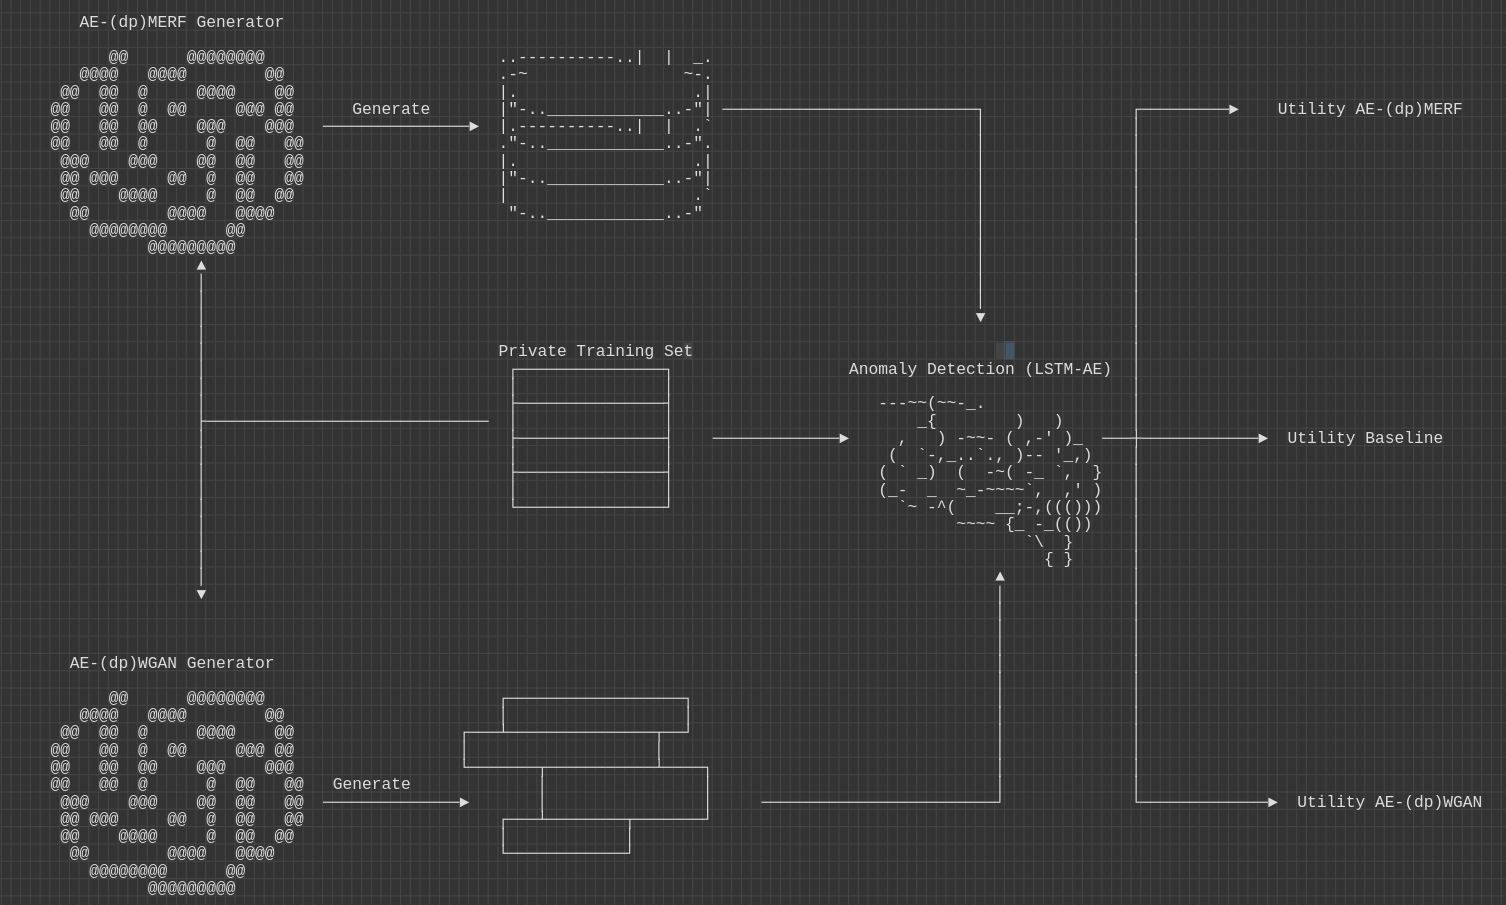
\includegraphics[scale=0.28]{str.png}
    \end{figure}
\end{frame}

\begin{frame}{Structure}
    \begin{enumerate}
        \item<1-> Train \alert{baseline model} for anomaly detection only on regular heartbeat data using an LSTM-AE.
        \item<2->  \alert{Generate heartbeat} data using two approaches:
        \begin{itemize}
            \item<2-> [--] AE-(dp)MERF
            \item<2-> [--] AE-(dp)WGAN
        \end{itemize}
        \item<3->  Train LSTM-AE for \alert{anomaly detection on synthetic data} and \alert{test on real}.
        \item<3-> Assess \alert{utility} by measuring performance for anomaly detection (Accuracy, precision, recall, F1). 
        \item<4->  \alert{Contaminate} training data with anomalous heartbeats and repeat.
    \end{enumerate}
\end{frame}




	\section{Dataset: MITBIH ECG data}
\begin{frame}{Heartbeat Arrhythmia}
    \begin{figure}
        \centering
        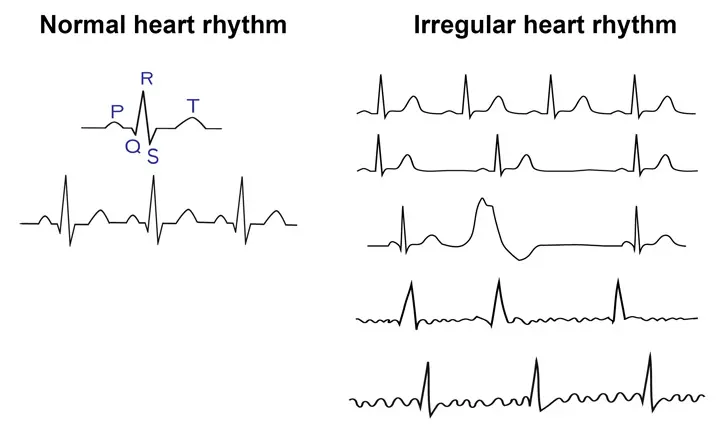
\includegraphics[scale=0.3]{images/heartbeat_arr.png}
        \caption[]{Different heartbeat arrhythmias \footnote{source: https://www.parkwayshenton.com.sg/health-plus/article/arrhythmia-guide}}
        \label{fig:enter-label}
    \end{figure}
\end{frame}

\begin{frame}{Arrhythmia Detection as an Anomaly Detection Problem}
We treat the problem of detecting irregular heartbeats as an anomaly detection problem from machine learning based on the reconstruction error:
\begin{itemize}
    \item<2->  We train a model \alert{on regular heartbeats} that is able to reconstruct that regular heartbeat.
    \item<3->  Given an irregular heartbeat the model should give \alert{higher reconstruction error}.
    \item<4->  Based on an optimal \alert{threshold} for that error we classify this heartbeat as either regular or irregular.
\end{itemize}
    \onslide<5>{Two reasons for this semi-supervised approach: high class imbalancy and no need for labelling.}
\end{frame} 

\begin{frame}{Baseline Model}
    Model is a LSTM-AE that is trained only on normal samples with the goal to reconstruct normal samples. The classification is made based on the reconstruction error.
    \begin{columns}
        \begin{column}{0.48\textwidth}
        \begin{figure}
            \centering
            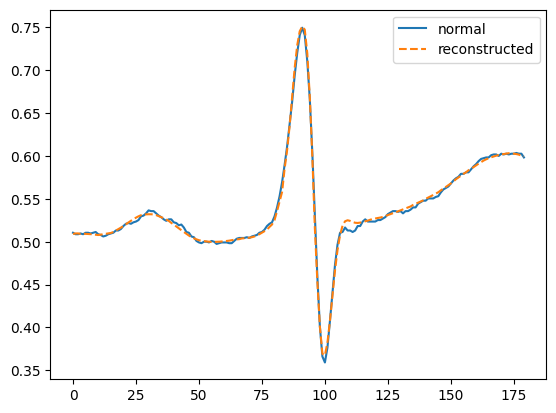
\includegraphics[scale=0.3]{images/rec_normal.png}
            \caption{reconstruction on normal sample \phantom{asdfsadf}}
            \label{fig:enter-label}
        \end{figure}
    \end{column}
    \begin{column}{0.48\textwidth}
        \begin{figure}
            \centering
            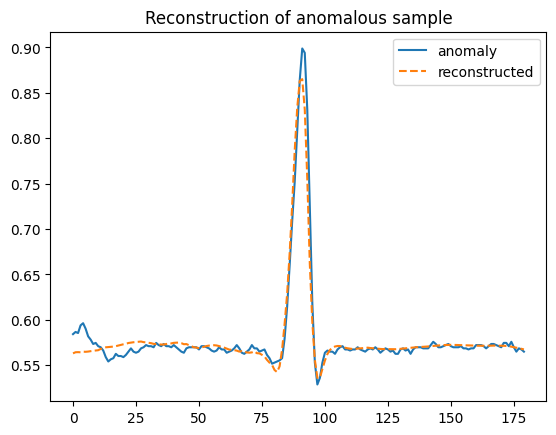
\includegraphics[scale=0.3]{images/rec_anom.png}
            \caption{reconstruction on anomalous sample}
            \label{fig:enter-label}
        \end{figure}
    \end{column}
    \end{columns}
\end{frame}

\begin{frame}
    \frametitle{Classification based on Reconstruction Error}

    \begin{columns}
        \begin{column}{0.48\textwidth}
        \begin{figure}
            \centering
            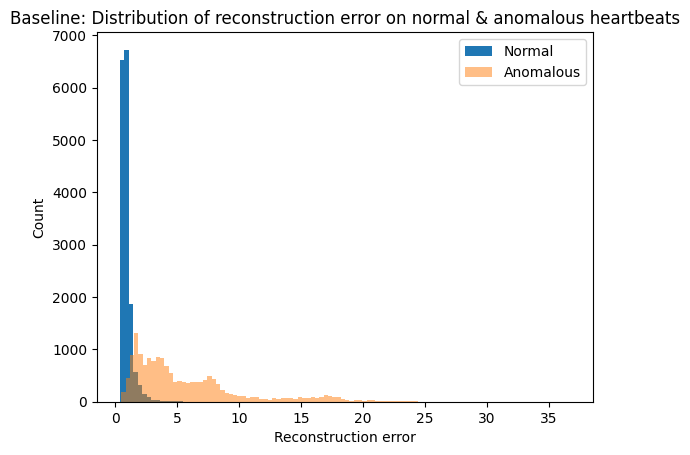
\includegraphics[scale=0.3]{hist_threshold_baseline.png}
            \caption{Distribution of reconstruction error on regular \& anomalous samples}
        \end{figure}
    \end{column}
    \begin{column}{0.48\textwidth}
        We can clearly see a \alert{difference in error distribution} for regular and anomalous samples. We choose the \alert{threshold that maximises the classification} accuracy.
    \end{column}
    \end{columns}

\end{frame}

	\section[(Time Series) Data generation]{(Time Series) Data generation}\label{chapter3}
\subsection{Overview}
    \begin{itemize}
        \item Data generation in general
        \item what is special about time series
        \item what about Privacy
        \item choice of models
    \end{itemize}

Time series data are sequences of data points in which there is a notion of time or ordering. Unlike tabular data, where each column corresponds to one feature, but it does not matter in which order one treats the different features. Time series are ubiquitous, common examples include weather data, financial transactions, energy consumption over time, stock prices etc.

We have chosen two architectures from the state of the art, that we will adapt to work on time series data. The first model is an example of a feature-based method, where a simple generative model is trained to map from a noise distribution to the data distribution. This is done by comparing the features of the synthetic data (or a suitable transformation thereof) with those of the original data. One particular instance of this class, DP-MERF \parencite{dpmerf}, has shown to give efficient and accurate results. Making this algorithm differentially private is straight-forward, since the loss function here can be separated into a term that is dependent on the original data and one that is not. So one only needs to introduce differential private noise to the data-dependent term once.


The second model follows a GAN-based approach. GANs introduced by Goodfellow et. al ???REF have been studied extensively in recent works as they have shown promising results in the field of image generation ??REF. They consist of two networks, a generator and a discriminator, where those two networks play a zero-sum game: the generator aims to generate authentic data whereas the discriminator aims to distinguish between generated and real data.


\subsection{DP-MERF}

DP-MERF \parencite{dpmerf} is an efficient all purpose data generation algorithm that is based on minimising the so-called Maximum Mean Discrepancy (MMD) between the real and the synthetic data distributions. It employs a so-called kernel mean embedding to transform the underlying probability distribution of the original data into a reproducing kernel hilbert space (RKHS). The distance between two distributions in the RKHS is then measured by the MMD. The authors mainly verified their results using tabular data like ????, but also image data, notably the MNIST ???CITE data set. It has not been used for time series data, but we will consider this data generation for generating time series data in this thesis, because according to a recent survey \parencite{hu2023sok}, DP-MERF delivers the best all purpose data generation performance.

\subsubsection{Maximum Mean Discrepancy}
There are different ways to measure the "distance" between two distributions $P$ and $Q$. On popular metric is the Maximum Mean Discrepancy (MMD) between $P$ and $Q$, where the random variables are projected into another feature space and the expected values are compared to each other in this space.

\begin{definition}[MMD]
    Let $\phi: \mathcal{X} \rightarrow \mathcal{H}$, where $\mathcal{H}$ is a reproducing kernel hilbert space (RKHS) and $P$ and $Q$ some distributions over $\mathcal{X}$ and random variables $X \sim P$, $Y \sim Q$ given. Then the Maximum mean Discrepancy is defined as:
    \begin{align}
        MMD(P,Q)=|| \mathbb{E}[\phi(X)] - \mathbb{E}[\phi(Y)] ||_\mathcal{H}
    \end{align}
\end{definition}

Some "easy" features maps $\phi$ are for example:
\begin{ex}
    Let $P$ and $Q$ some distributions over $\mathcal{X}$ and random variables $X \sim P$, $Y \sim Q$ given.
    \begin{itemize}
        \item \textbf{Identity kernel}: $\mathcal{X}=\mathcal{H}=\mathbb{R}^d$ and $\phi(x)=x$, then we have:
        \begin{align}
            MMD(P,Q) &= || \mathbb{E}[\phi(X)] - \mathbb{E}[\phi(Y)] ||_\mathcal{H} \nonumber \\
            &= || \mathbb{E}[X] - \mathbb{E}[Y] ||_{\mathbb{R}^d}
        \end{align}
        So we only compare the two distributions in terms of their means. 

        \item \textbf{Quadratic kernel}: $\mathcal{X}=\mathbb{R}$ $\mathcal{H}=\mathbb{R}^2$ and $\phi(x)=(x, x^2)$, then we have:
        \begin{align}
            MMD(P,Q) &= || \mathbb{E}[\phi(X)] - \mathbb{E}[\phi(Y)] ||_\mathcal{H} \nonumber \\
            &= || \mathbb{E}[(X, X^2)] - \mathbb{E}[(Y, Y^2)] ||_\mathcal{H} \nonumber \\
            &= || \begin{pmatrix}
                \mathbb{E}[X] \\ \mathbb{E}[X^2]
            \end{pmatrix} - \begin{pmatrix}
                \mathbb{E}[Y] \\ \mathbb{E}[Y^2]
            \end{pmatrix} ||_{\mathbb{R}^2} \nonumber \\
            &= \sqrt{(\mathbb{E}[X] - \mathbb{E}[Y])^2 - (\mathbb{E}[X^2] - \mathbb{E}[Y^2])^2}
        \end{align}
        So here we compare the two distributions in terms of their means and their variance (or first and second moments respectively).
        \item \textbf{Gaussian kernel} ????
    \end{itemize}
\end{ex}

Now instead of computing a possibly high or even infinite dimensional transformation $\phi$ one can use the well-known kernel trick ????REF. Let $k(x,y)=<\phi(x), \phi(y)>_{\mathcal{H}}$ be a kernel with corresponding reproducing kernel hilbert space $\mathcal{H}$, then the computation of the MMD simplifies to:

\begin{align}
    MMD^2(P,Q) &= || \mathbb{E}[\phi(X)] - \mathbb{E}[\phi(Y)] ||^2_\mathcal{H} \nonumber \\
    &= <\mathbb{E}[\phi(X)], \mathbb{E}[\phi(X')]> - <\mathbb{E}[\phi(X)], \mathbb{E}[\phi(Y)]> - <\mathbb{E}[\phi(Y)], \mathbb{E}[\phi(X)]> \nonumber \\ &\phantom{mmmmmmmmmmmmmmmmmmmm}+ <\mathbb{E}[\phi(Y)], \mathbb{E}[\phi(Y')]> \nonumber \\
    &= \mathbb{E}[<\phi(X), \phi(X')>] - 2 \mathbb{E}[<\phi(X), \phi(Y)>] + \mathbb{E}[<\phi(Y), \phi(Y')>] \nonumber \\
    &= \mathbb{E}[k(X,X')] - 2 \mathbb{E}[k(X,Y)] + \mathbb{E}[k(Y,Y')]
\end{align}

Where we introduced independent random variables $X,X' \sim P$, $Y,Y' \sim Q$.

\subsubsection{Random Fourier Features}

Now given a training data set $X_m = \{x_i\}_{i=1}^m \sim P$ and a synthetic data set $X'_m = \{x_i\}_{i=1}^m \sim Q$ we can estimate their $MMD^2$ by estimating the expected value with a mean estimate:

\begin{align} \label{eq:mmd}
    \widehat{MMD}^2(X_m, X'_m) = \frac{1}{m^2} \sum_{i,j=1}^m k(x_i,x_j) + \frac{1}{m^2} \sum_{i,j=1}^m k(x'_i,x'_j) - \frac{2}{m^2} \sum_{i,j=1}^m k(x_i,x'_j)
\end{align}
Unfortunately, this will require $\mathcal{O}(m^2)$ computations which grows quadratically in the number of samples. This will be too big for a large training data set. As a remedy, the authors of \parencite{dpmerf} propose to use Random Fourier Features based on a paper from 2007 \parencite[see][]{rff}, to approximate the kernel $k$ using its fourier transform and Monte-Carlo-Simulation.

\begin{align}
    k(x,y) \approx \hat{\Phi}(x)^T \hat{\Phi}(x')
\end{align}
where $\hat{\Phi}(x) \in \mathbb{R}^D$ and $\hat{\Phi}_j(x) = \sqrt{\frac{2}{D}} cos (\omega_j^T x)$.

If we sample $w_j \sim \mathcal{N}$ from the Gaussian distribution, we are approximating the gaussian kernel.

Now we can approximate equation \ref{eq:mmd} using those random fourier features:

\begin{align} \label{eq:rff}
    \widehat{MMD}^2_{RFF}(X_m, X'_m) &\approx \frac{1}{m^2} \sum_{i,j=1}^m \hat{\Phi}(x_i)^T \hat{\Phi}(x_j') + \frac{1}{m^2} \sum_{i,j=1}^m \hat{\Phi}(x_i)^T \hat{\Phi}(x_j') - \frac{2}{m^2} \sum_{i,j=1}^m \hat{\Phi}(x_i)^T \hat{\Phi}(x_j') \nonumber \\
    &= || \frac{1}{m} \sum_{i=1}^m \hat{\Phi}(x_i) - \frac{1}{m} \sum_{j=1}^m \hat{\Phi}(x_j') ||_\mathcal{H}^2
\end{align}

more stuff: https://gregorygundersen.com/blog/2019/12/23/random-fourier-features/

\subsubsection{Vanilla DP-MERF}
We can now introduce the version of DP-MERF presented in \parencite{dpmerf}. Let $G_\theta$ denote a generative neural network with parameters $\theta$, i.\ e.\ given input $z \sim p(z)$ from some known probability distribution $p(z)$ we obtain a synthetic sample through $x' = G_\theta(z)$. We denote the distribution of the synthetic data samples by $Q$. Further, let $X_m = \{x_i\}_{i=1}^m \sim P$ be our training data with true distribution $P$. By minimising 
\begin{align}
    \widehat{\theta} &= \argmin_\theta \widehat{MMD}^2_{RFF}(P, Q) \nonumber \\
    &\overset{\ref{eq:rff}}{=} \argmin_\theta || \frac{1}{m} \sum_{i=1}^m \hat{\Phi}(x_i) - \frac{1}{m} \sum_{j=1}^m \hat{\Phi}(x_j') ||_2^2 \nonumber \\
    &= \argmin_\theta || \hat{\mu}_P - \hat{\mu}_Q ||_2^2
\end{align}

where we introduced notation $\hat{\mu}_P = \frac{1}{m} \sum_{i=1}^m \hat{\Phi}(x_i)$ and $\hat{\mu}_Q = \frac{1}{m} \sum_{i=1}^m \hat{\Phi}(x'_i)$. The DP version is obtained by observing that the original data set is entering the equation only through $\hat{mu}_P$ so we have to introduce noise only in this term by adding gaussian noise:
\begin{align}
    \tilde{\mu}_p = \hat{\mu}_P + \mathcal{N}(0, \sigma^2 I)
\end{align}
We choose $\sigma$ according to definition \ref{def:gm}. For a given privacy level $(\epsilon, \delta)$ we need to compute the sensitivity $\Delta_{\hat{\mu}_P}$. There is an upper bound since we have by definition:
\begin{align}
    \Delta_{\hat{\mu}_P} &= \max_{\substack{X_m,X_m' \\ ||X_m-X_m'||_1=1}} || \frac{1}{m} \sum_{i=1}^m \hat{\Phi}(x_i) - \frac{1}{m} \sum_{j=1}^m \hat{\Phi}(x_j') ||_2 \nonumber \\
    &= \frac{1}{m} \max_{x_m \neq x'_m} || \hat{\Phi}(x_m) - \hat{\Phi}(x'_m)||_2 \nonumber \\
    &\overset{\Delta \neq}{\leq} \frac{1}{m} \max_{x_m \neq x'_m} || \hat{\Phi}(x_m) ||_2 + ||\hat{\Phi}(x'_m)||_2 \nonumber \\
    &\leq \frac{2}{m} 
\end{align}
where in the second equality we assumed without loss of generality that $X_m$ and $X_m'$ differ only in their last element, so that the other summands cancel each out and in the last inequality we are using the fact that $||\hat{\Phi}(\cdot)||_2 \leq 1$.


\subsection{RTSGAN} 

\subsubsection{Review: GANs}
Generative adversarial networks (GAN) were first introduced in 2014 by Goodfellow et. al in \parencite{gan_og} as an unsupervised learning algorithm for generative modelling. Since then it has been used extensively in image generation, where it excels at generating high-resolution images. The original paper proposes a joint training of two machine learning models to output $\hat{p}_{model}$, usually neural networks, to implicitly model the unknown data distribution $p_{data}$ of a given training set. 

Therefore, the first network denoted by $G$, commonly referred to as the generator, is able to sample from $\hat{p}_{model}$ by finding a mapping from some random noise $z$ and maps it to a sample $G(z; \theta_G)$ following $\hat{p}_{model}$. $G$ is parametrised by a set of weights $\theta_G$. The second model denoted by $D$, commonly referred to as the discriminator, aims to distinguish generated samples $\hat{x}= G(z,\theta_G)$ from real samples $x$, which can be treated as a binary classification model. The output $D(x; \theta_D)$ then is an estimate whether $x$ is a real sample, i. e. sampled from $p_{data}$ or fake, i. e. sampled from $\hat{p}_{model}$ respectively. Similarly, $D$ is parametrised by $\theta_D$.

During training the weights $\theta_D$ and $\theta_G$ are adjusted in order to minimise or maximise a certain loss:
\begin{itemize}
    \item $D$ is trained to maximise the probability of correctly classifying real and generated samples.
    \item $G$ is trained to minimise the probability that $D$ identifies the generated samples.
\end{itemize}

This leads to the following minmax loss:
\begin{align} \label{eq:gan_loss}
    \min_G \max_D \mathbb{E}_x[\log D(x)] + \mathbb{E}_z[1-D(G(z))]
\end{align}
The training is done sequentially, i. e. in every epoch we first update the discriminator's weights using a some type of gradient descent that maximises equation \ref{eq:gan_loss}. Then the generator's weights are adjusted so that it minimises equation \ref{eq:gan_loss}. This optimisation can be regarded as a zero-sum game from game theory. 

Although theoretical results for convergence where obtained in the original paper by Goodfellow et al., in practise GANs suffer from stability issues coming from exploding or vanishing gradients and mode-collapse \parencite[see][for in-depth review]{gui2020review,jabbar2020survey}. Thus, modifications to the loss function and training process that aim to stabilise training where developed, e. g. WGAN using the Wasserstein loss \parencite{arjovsky2017wasserstein}.

In light of privacy concerns, standard GAN architectures without any formal privacy guarantees do not preserve any meaningful privacy of the training data. This negative results has been confirmed in \parencite{lin2021privacy,stadler2022synthetic}. Hence, a dedicated privacy mechanism has to be used. In particular, we will ``privatise'' the GAN architecture by using a DP-SGD when training the discriminator, similar to \parencite{xie2018differentially}.

\subsubsection{Time series Generation with RTSGAN}
The authors in \parencite{pei2021towards} propose a hybrid approach that employs a similar idea to our proposed AE-(DP)MERF algorithm; it combines an autoencoder architecture to learn a latent space and generates data within that space with a WGAN network.

\begin{figure}[h]
    \centering
    
\includegraphics[scale=0.5]{../images/placeholder.png}
    \caption[]{Architecture of RTSGAN from \parencite{pei2021towards}}
\end{figure}

The authors also implement a mechanism to handle missing values, but we will not concern about this issue for the scope of this thesis.
\begin{itemize}
    \item \underline{Autoencoder component:} A gated recurrent unit (GRU) is used for both the encoder and the decoder. The encoder transforms the time series into a vector of fixed size in the latent space. This latent representation is then fed into the decoder which aims to reconstruct the time series from the latent space.
    \item \underline{Generator component} The generator is based on the WGAN architecture. The main differences to a regular GAN lie in the loss function which is based on the so-called Wasserstein-1 distance and penalty term. Further, a Lipschitz-constraint is imposed on the discriminator through this penalty term.
    \begin{align} \label{eq:wgan_loss}
        \min_G \max_{D \in \mathcal{D}} \mathbb{E}_x[\log D(x)] - \mathbb{E}_z[D(G(z))] + \lambda \mathbb{E}_z [ (||\nabla_z D(G(z))||_2 - 1)^2]
    \end{align}
    where $\mathcal{D}$ denotes the set of 1-Lipschitz functions \footnote[1]{a differentiable function is 1-Lipschitz if and only if its derivative is bounded in norm by 1}). To impose this constraint, the authors chose to impose a penalty on the gradients as suggested in \parencite{arjovsky2017wasserstein}.
\end{itemize}

	\clearpage

	\fancyhead[L]{APPENDIX}
	\section*{Appendix}
	\addcontentsline{toc}{section}{Appendix}
	\section*{Appendix}

	\clearpage

	\pagestyle{fancy}
	\fancyhead[L]{REFERENCES}
	\fancyfoot[R]{\thepage}
	\printbibliography[heading=bibintoc, title=References]
\end{document}
